\chapter{Introduction}
\label{chap:intro}

Today's general purpose file systems fail to utilize the full bandwidth of the
underlying hardware.
Widely used inode-based file systems, such as ext4, XFS, and Btrfs, can write
large files at near disk bandwidth,
but typically create small files at less than 3\% of the disk bandwidth~\citep{betrfs2}.
Similarly, these file systems can read large files at near disk bandwidth,
but traversing directories with many small files is slow, and the performance
degrades when the file system ages~\citep{betrfs3}.

At the heart of this issue is how file systems organize metadata and data
on disk.
The most common design pattern for modern file systems is to use multiple layers
of indirection.
The inode number of a file or directory connects the name of an entry in the
parent directory to its metadata location on disk.
The metadata of an inode contains extents that describe the physical location
of data at different offsets.
Indirection simplifies the implementation of file systems.
However, indirection doesn't impose any constraints on how metadata and
data are placed on disk.
In the worst case, the metadata of entries under a directory and the data of
a file can end up scattered over the disk.
Because random I/Os are much slower than sequential I/Os on disks,
directory traversals and file creations can be extremely slow.
Heuristics, such as cylinder groups~\citep{ffs1}, are designed to mitigate this
problem.
However, after disk space is allocated and freed over file system aging,
the free space on disk becomes scattered, making such heuristics
ineffective in the worst case.

One attempt to solve the problem of file creations is the log-structured file
system~\citep{lfs}.
The log-structured file system treats the whole disk as a log,
and all write operations, including file creations, become log appends,
which are written to the underlying disk sequentially.
Therefore, file creations are much faster on the log-structured file system.
However, the log cleaner in a log-structured file system has severe impact on
performance~\citep{lfsbsd}, especially when the log is full.

Alternatively, a file system can put metadata and data in
write-optimized dictionaries (WODs).
WODs, such as the LSM-tree~\cite{lsm},
consist of multiple levels whose sizes grow exponentially.
Writes are treated as log appends to the lowest level, and gradually merged to
higher levels in batches.
Because all data are written in batches, the amortized cost of each write is
much smaller in WODs,
despite the fact that each write is written multiple times.
Thus, file creations are much faster on WOD-based file systems, such as
TableFS~\citep{tablefs}.

However, previous WOD-based file systems are still inode-based.
In other words, these file systems use inode numbers as indexes for
metadata and data.
Because the inode number of a file or directory doesn't change once allocated,
after file deletions and creations over file system aging,
files in the same directory can be assigned with inode numbers that are
irrelevant to each other in the worst case.
In such a scenario, the file system is unable to group the inodes in the
same directory close to each other in the WOD.
Therefore, a directory scan in inode-based, WOD-based file system can still
result in many random I/Os in the worst case.

An alternative design is to use full-path indexing upon WODs in a file system,
known to have good performance on nearly all operations.
A full-path-indexed file system indexes metadata and data
using the full-paths of the file or directory,
and sorted the full-paths in depth-first-search order,
that is, lexicographic order by the full-paths of files and directories.
With full-path indexing, metadata and data under one directory are close to each
other in the key space, which, combined with the sorted order maintained by
WODs, leads to good locality and fast directory traversals.
Prior work~\citep{betrfs1,betrfs1tos,betrfs2,betrfs2tos,betrfs3} of this design
realizes efficient implementation of many file-system operations, such as random
writes, file creations and directory traversals,
but a few operations have prohibitively high overheads.

The Achilles' heel of full-path indexing is the performance of namespace
operations, in particular, renaming large files and directories.
In inode-based file systems,
renaming a file or directory is just a pointer swing,
moving an entry from one directory to another directory,
without touching the file or directory being renamed.
However, with full-path indexing, renaming a directory involves changing the
full-paths of all files and directories under it,
updating keys of the metadata and data and moving them in the key space.
Competitive performance for namespace operations infull-path-indexed file
systems should complete in an I/O-efficient manner.

\begin{figure}[t]
    \centering
    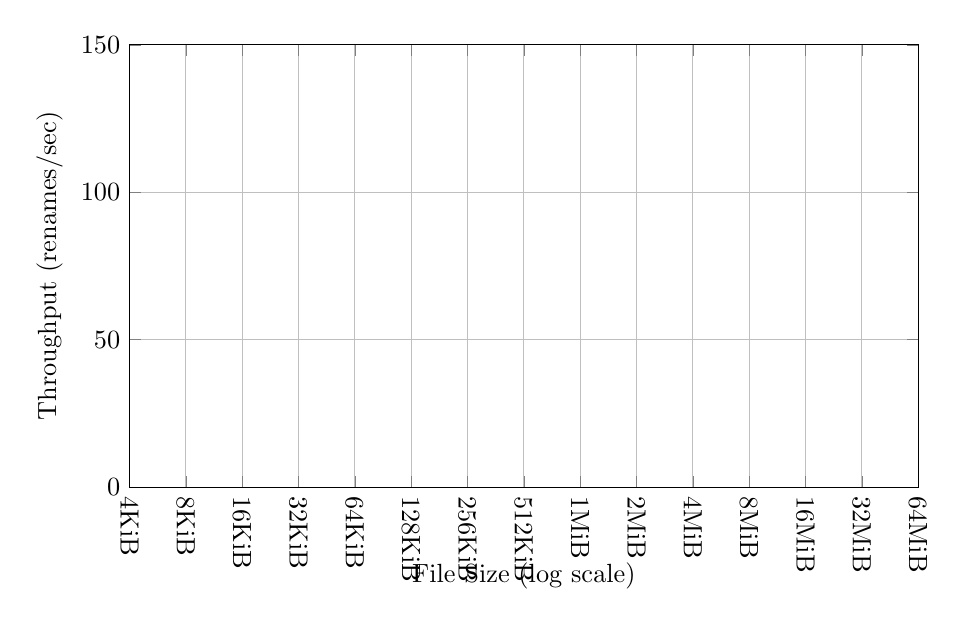
\begin{tikzpicture}[yscale=0.95, xscale=0.95]
        \begin{axis}[
                xlabel={File Size (log scale)},
                x label style={at={(axis description cs:0.5,-0.15)},anchor=north},
                ylabel={Throughput (renames/sec)},
                xmin=12,
                xmax=26,
                xtick={12,13,14,15,16,17,18,19,20,21,22,23,24,25,26},
                xticklabels={4KiB,8KiB,16KiB,32KiB,64KiB,128KiB,256KiB,512KiB,1MiB,2MiB,4MiB,8MiB,16MiB,32MiB,64MiB},
                xticklabel style={rotate=270, anchor=west},
                ymin=0,
                ymax=150,
                grid=major,
                scaled x ticks=false,
                scaled y ticks=false,
                legend columns=4,
                legend cell align=left,
                height=.618\linewidth,
                width=\linewidth,
            ]
            \addFileRenamePlot{ext4};
            \addFileRenamePlot{btrfs};
            \addFileRenamePlot{xfs};
            \addFileRenamePlot{zfs};
            \addFileRenamePlot{nilfs2};
            \addFileRenamePlot{betrfs3-max};
        \end{axis}
    \end{tikzpicture}
    \caption[The performance of file renames in full-path-indexed file systems]{\label{fig:file_rename_intro}
        Throughput of renaming a file of different sizes (higher is better).
        The performance of full-path-indexed \betrfsThree
        degrades when the file being renamed becomes larger.}
\end{figure}

However, prior work mainly focuses on the schema level of the file system, i.e.,
how metadata and data are keyed and indexed in WODs.
Renames on those full-path-indexed file systems are implemented by fetching all
related key/value pairs of metadata and data,
inserting them back with updated keys, and deleting old key/value pairs.
In such a design, a file system rename needs to call several operations for each
affected full-path names, leading to bad performance,
especially when the file or directory being renamed is large.
Figure~\ref{fig:file_rename_intro} compares the throughput of file renames in
different file systems.
The benchmark renames a file of different sizes 100 times, each followed by a
\texttt{fsync} of the parent directory.
Except full-path-indexed \betrfsThree, all file systems are inode-based.
As the file size changes, these inode-based file systems have relatively
stable rename throughput.
In contrast, file renames in full-path-index \betrfsThree become slower and
slower when the file size grows,
because the file system needs to update more key/value pairs
(full-path-indexed \betrfsThree stores each 4KiB block of a file as
a key/value pair).

This dissertation presents I/O-efficient implementations of namespace operations
in a full-path-indexed, write-optimized file system.
Specifically, though full-path indexing limits possible changes on the schema
level, we observe that it can make all full-path names under a directory
contiguous in the key space.
And the underlying WODs, \bets, have a tree structure, which makes it possible
to move a contiguous key range in a subtree efficiently.
Therefore, we dig into the underlying \bets, and implement a new operation,
range-rename, that completes file system renames with a bounded number of I/Os.
Moreover, the contiguity in the key space enables namespace operations that are
difficult in inode-based file systems.
In particular, we expand the range-rename operation into the range-clone
operation, which can complete file or directory clones efficiently.

The primary contribution of this dissertation is to show that there is no
trade-off between efficient namespace operations and locality.
One can implement efficient renames in a full-path-indexed, write-optimized
file system while keeping the locality ensured by full-path indexing.
In fact, with full-path indexing, one can implement namespace operations that
are difficult in inode-based file systems, such as directory clones.

Chapter~\ref{chap:bg} describes the necessary background of this dissertation.
It starts with a presentation of the write-optimized \bets,
showing the idea of write-optimization.
Then, it describes full-path-indexed \betrfs and relative-path-indexed \betrfs.
The full-path-indexed \betrfs shows the benefit of full-path indexing and
write-optimization, but suffers from slow renames.
The relative-path-indexed \betrfs has good rename performance, but breaks the
full-path indexing and taxes other operations for efficient renames.

Chapter~\ref{chap:rename} presents the range-rename operation on \bets.
All key/value pairs in the \bet whose keys have a certain prefix are updated to
have keys with another prefix after the range-rename operation.
This is done efficiently through two techniques,
\textbf{key lifting} and \textbf{tree surgery}.
And with efficient range-rename, full-path-indexed \betrfs can implement file
system renames efficiently.

Chapter~\ref{chap:clone} expands the range-rename operation into the
range-clone operation.
It first shows how to implement the range-clone operation with range-rename
techniques by transforming \bets into \bedags.
Then, it introduces a new type of messages to \bedags, \goto messages.
The \goto message works like other messages in \bedags,
fitting the range-clone operation into write-optimization.
Full-path-indexed \betrfs can use the range-clone operation to implement both
file or directory renames and clones.

Chapter~\ref{chap:eval} evaluates the implementation.
It compares full-path-indexed \betrfs with range-rename or range-clone to
widely used file systems on micro and application benchmarks.
It also puts a particular focus on benchmarking namespace operations.

Chapter~\ref{chap:related} discusses previously published work related to
this work.
It organizes related work by topic, and talks in detail about work that is
closely related to this work.

Chapter~\ref{chap:conclusion} summarizes and concludes the dissertation.

